\subsection{Submit Problem}

\begin{frame}
\begin{figure}[htbp]
\begin{center}
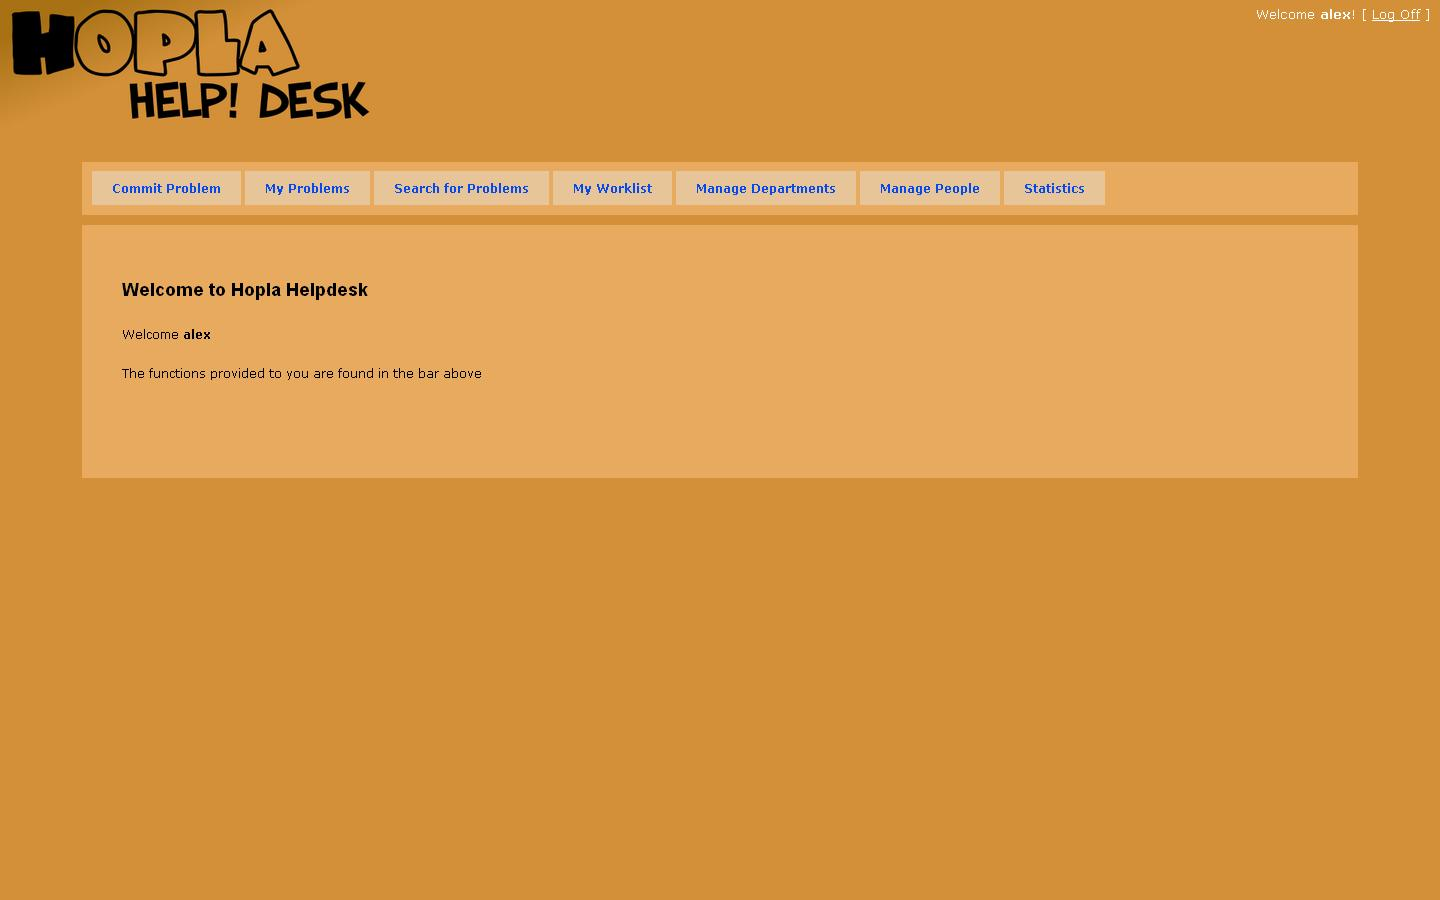
\includegraphics[width=\textwidth]{input/search/home.JPG}
%\caption{default}
%\label{default}
\end{center}
\end{figure}

\end{frame}

\begin{frame}

\begin{figure}[htbp]
\begin{center}
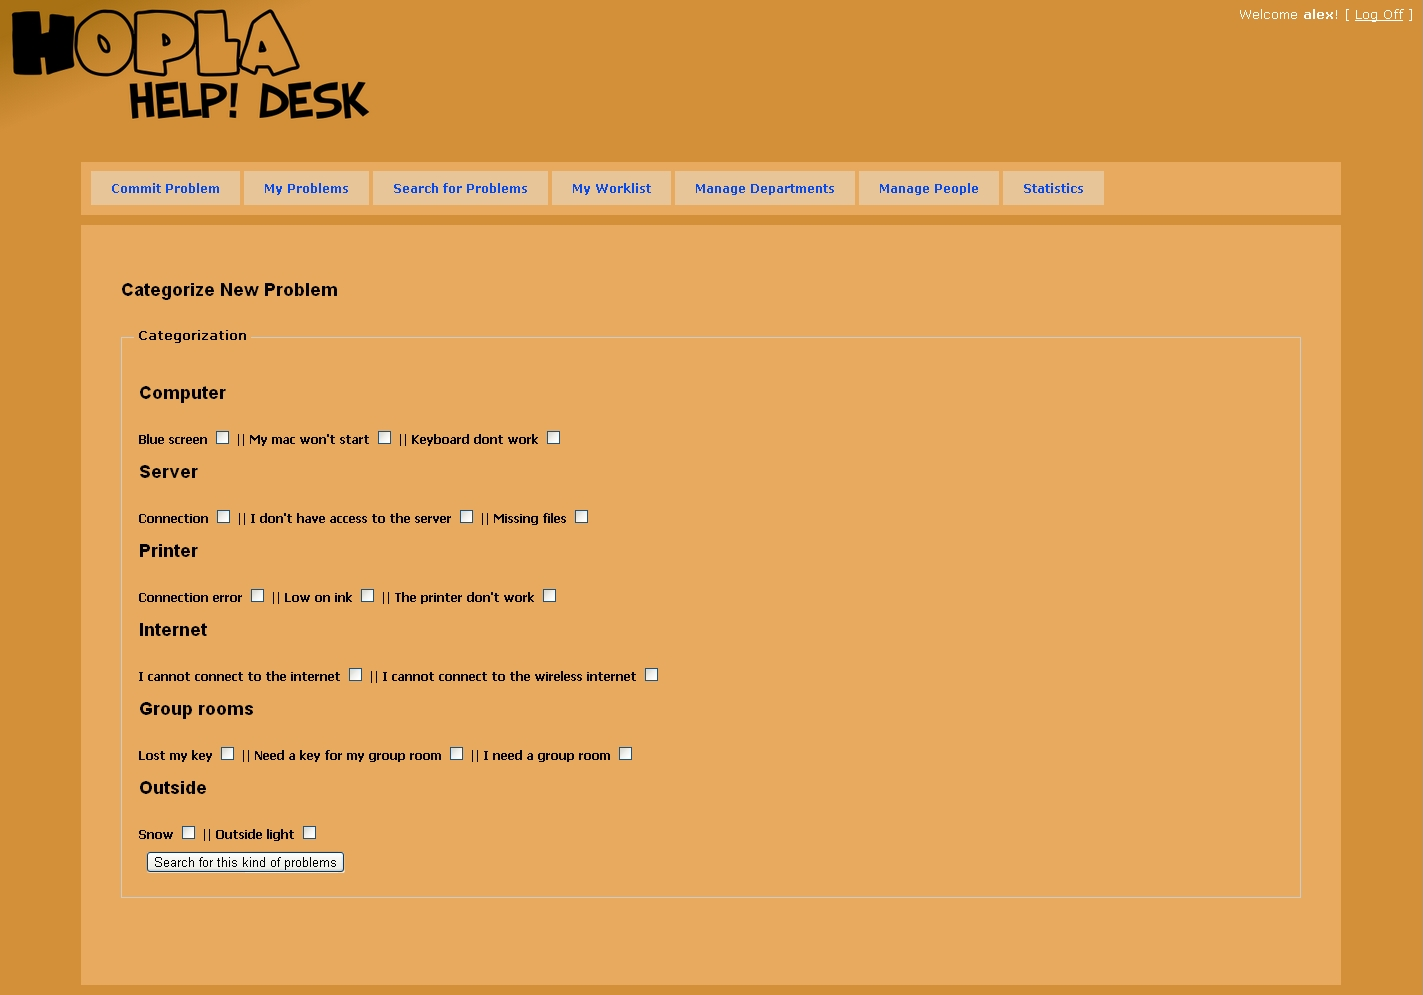
\includegraphics[width=\textwidth]{input/search/commit.png}
%\caption{default}
%\label{default}
\end{center}
\end{figure}

\end{frame}

\begin{frame}

\begin{figure}[htbp]
\begin{center}
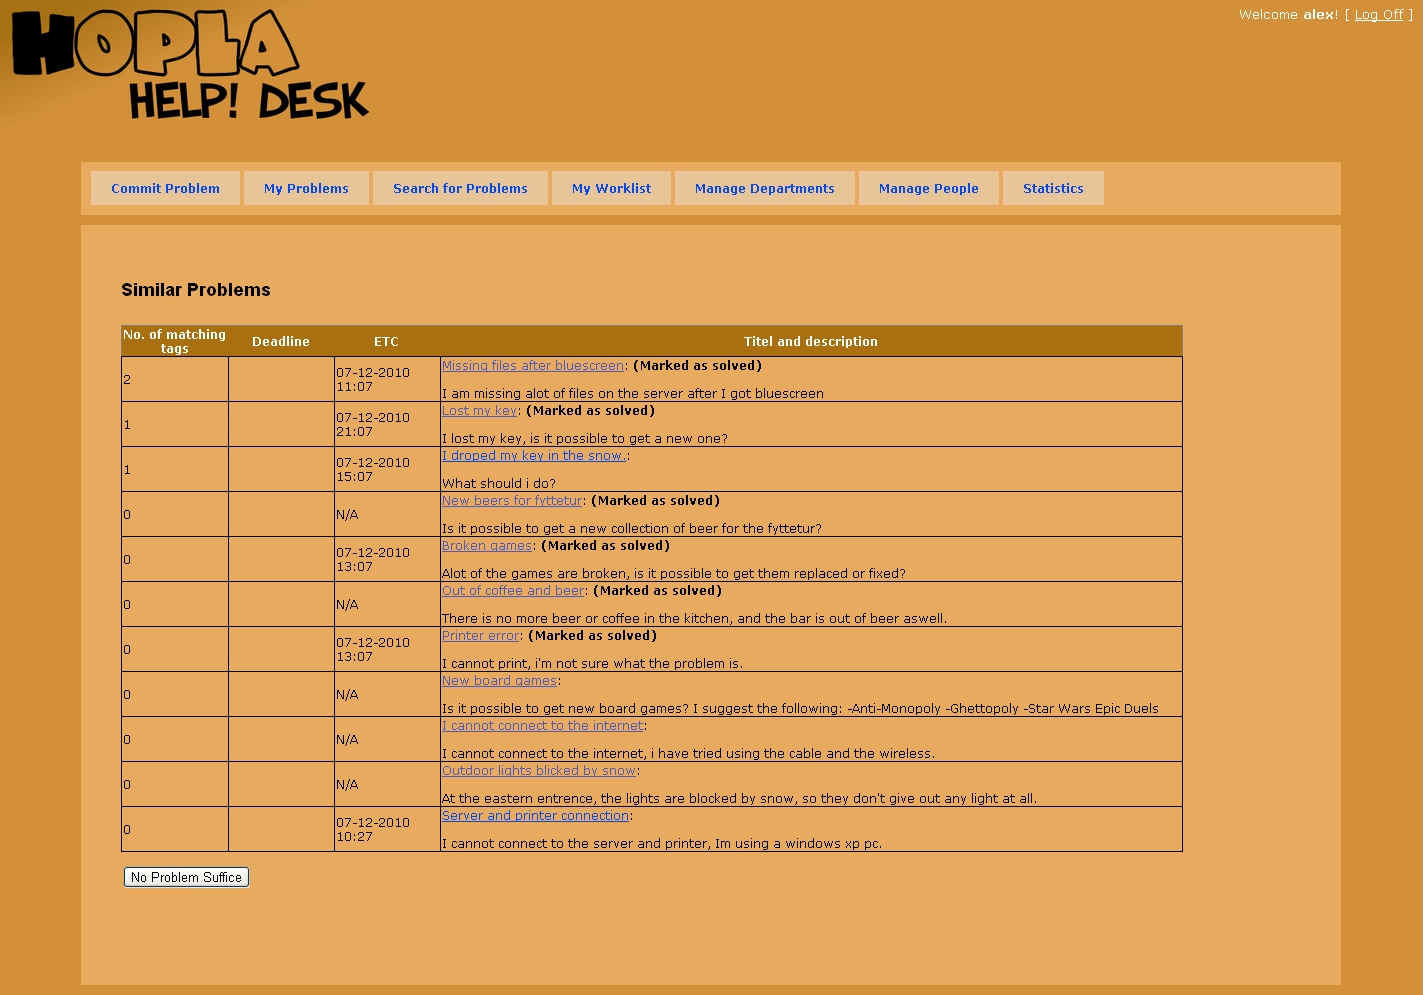
\includegraphics[width=\textwidth]{input/search/similarProblems.png}
%\caption{default}
%\label{default}
\end{center}
\end{figure}

\end{frame}

\begin{frame}

\begin{figure}[htbp]
\begin{center}
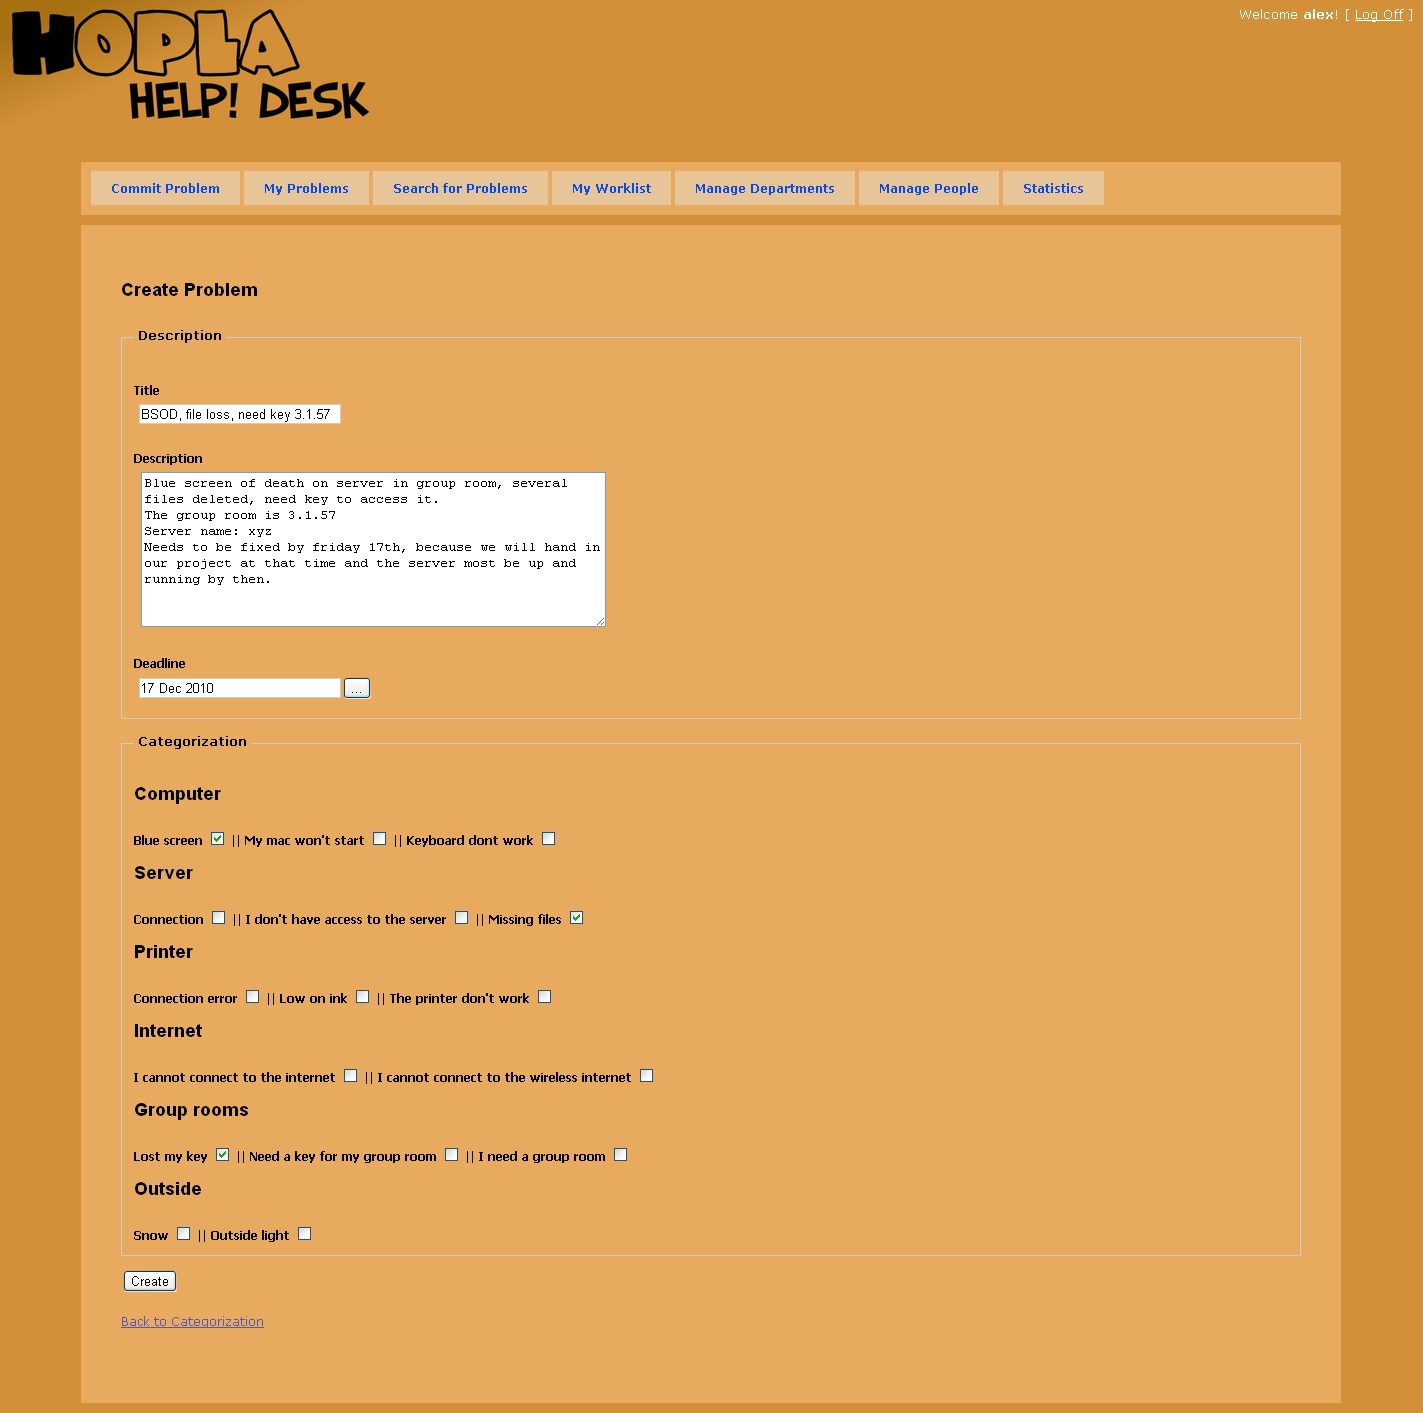
\includegraphics[width=\textwidth]{input/search/newProblem.png}
%\caption{default}
%\label{default}
\end{center}
\end{figure}

\end{frame}
% The interresting here is the search, we try search a set of problems



\subsubsection{Search}
\begin{frame}{The Search}
\begin{itemize}
\item Tags to search: Computer + Blue screen
\item Minimum number of problems to find: 3
\item Problems to search in 
\begin{itemize}
	\item Computer \only<2>{(One match)}
	\item Blue screen  \only<2>{(One match)}
	\item Computer + Blue screen  \only<2>{(Two matches)}
	\item Computer + Blue screen + Internet  \only<2>{(Two matches and one unrelated)}
	\item Computer + Internet  \only<2>{(One Math and one unrelated)}
	\item Internet  \only<2>{(No Match)}
	\end{itemize}
	\end{itemize}

\end{frame}


\subsubsection{Search}
\begin{frame}{The Search}
\begin{itemize}
	\item Result
\begin{itemize}
%First it finds where both is and sorts so the one with minumum number of tags is presented. 
\item Computer + Blue screen 
\item Computer + Blue screen + Internet
%then it removes the  Computer, as it is first.
\item Blue screen
\item Computer
\item Computer + Internet
% They get sorted ofter number og tags.
% IF minimum were higher Internet will be with as well
\end{itemize}\end{itemize}
\end{frame}

